\documentclass[a4paper]{article}

%% Language and font encodings
\usepackage[english]{babel}
\usepackage[utf8x]{inputenc}
\usepackage[T1]{fontenc}

%% Sets page size and margins
\usepackage[a4paper,top=3cm,bottom=2cm,left=3cm,right=3cm,marginparwidth=1.75cm]{geometry}

%% Useful packages
\usepackage{amsmath}
\usepackage{graphicx}
\usepackage[colorinlistoftodos]{todonotes}
\usepackage[colorlinks=true, allcolors=blue]{hyperref}
\usepackage{float}
\usepackage{algorithm}
\usepackage[noend]{algpseudocode}
\usepackage{listings}

\graphicspath{ {images/} }

\title{Peg Solitaire Backtracking Assignment}
% \author{}
% Update supervisor and other title stuff in title/title.tex

\begin{document}
\begin{titlepage}

\newcommand{\HRule}{\rule{\linewidth}{0.5mm}} % Defines a new command for the horizontal lines, change thickness here

\center % Center everything on the page
 
%----------------------------------------------------------------------------------------
%	HEADING SECTIONS
%----------------------------------------------------------------------------------------

\textsc{\LARGE University of the Witwatersrand}\\[1.5cm] % Name of your university/college
\textsc{\Large COMS3005: Advanced Analysis of Algorithms}\\[0.5cm] % Major heading such as course name
% \textsc{\large Minor Heading}\\[0.5cm] % Minor heading such as course title

%----------------------------------------------------------------------------------------
%	TITLE SECTION
%----------------------------------------------------------------------------------------
\makeatletter
\HRule \\[0.4cm]
{ \huge \bfseries \@title}\\[0.4cm] % Title of your document
\HRule \\[1.5cm]
 
%----------------------------------------------------------------------------------------
%	AUTHOR SECTION
%----------------------------------------------------------------------------------------
{\large \today}\\[2cm] % Date, change the \today to a set date if you want to be precise

\begin{minipage}{1\textwidth}
  \Large \emph By Bancroft, E. (879192)\\
  \Large \emph And Chalom, J. (711985)\\
\end{minipage}

% If you don't want a supervisor, uncomment the two lines below and remove the section above
%\Large \emph{Author:}\\
%John \textsc{Smith}\\[3cm] % Your name

%----------------------------------------------------------------------------------------
%	DATE SECTION
%----------------------------------------------------------------------------------------



%----------------------------------------------------------------------------------------
%	LOGO SECTION
%----------------------------------------------------------------------------------------

% \includegraphics[width=8cm]{title/logo.png}\\[1cm] % Include a department/university logo - this will require the graphicx package
 
%----------------------------------------------------------------------------------------

\vfill % Fill the rest of the page with whitespace

\end{titlepage}

% \lfoot{School of Computer Science and Applied Mathematics}
\clearpage
\setcounter{page}{1}
% \setcounter{section}{1}
\pagenumbering{arabic}

% \section*{Abstract}


\section{Introduction}
The purpose of the assignment is to implement and analyse a version of the Peg Solitaire game and the backtracking algorithm (to play the game to completion and return a valid path).

\section{Background}
Peg Solitaire is a board game which has a number of holes that can be filled with pegs. We have chosen to use the European/French style of board which has four extra positions for pegs on the board \ref{board}. In this style most of a grid has peg holes excluding three per corner. The aim of the game is to remove pegs until only one peg remains. This is the position one row directly above the central peg, a row above that and the left most peg in the top row. Moves are made when pegs jump over a peg and are placed in an open position. Then a peg which has been jumped over, is then removed. This move can happen in both horizontal and vertical directions. In the European variant, the game has three possible optimal terminal states. Its is possible to hit sub-optimal states where there are more pegs left on the board but no possible moves left \cite{harder}. 

% Have example moves and suboptimal states?
\begin{figure}[H]
	\centering
	\label{board}
	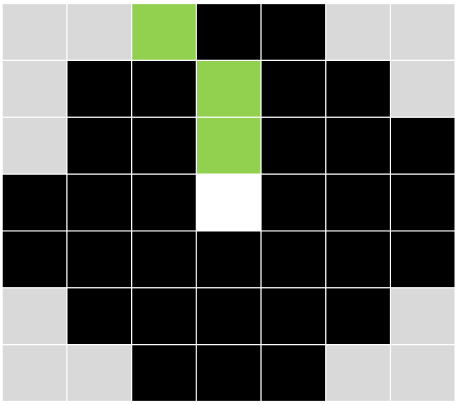
\includegraphics[width=.50\textwidth,scale=.50]{images/board}
	\caption{Diagram of an European Peg Solitaire Board Where the
				Black Squares Represent Peg Positions,
				Green Are Terminal Positions,
				Grey Are Not Positions and
				White is the Central Pixel.
			}
\end{figure}

% cite the wayback machine??
\noindent The backtracking algorithm is similar to a brute force approach to finding solutions to problems but is more systematic. It attempts to follow a logical series of decisions in solving these problems and when a block state occurs the algorithm will backtrack to previous decisions and choose different paths until a terminal (complete) state is reached. The full set of solutions to a problem can be found by continuing to run the algorithm until all paths have been searched but that is not always necessary.

\begin{algorithm}[H]
	\begin{algorithmic}[1]
		\Procedure{FindSolution}{\texttt{start, final, path}}
			\If {\texttt{start.numPegs <= final.numPegs}}
				\State \Return (start = final)
			\Else 
				\For{\texttt{each jump $J \in$ [0,n) x [0,m) x \{NORTH,EAST,SOUTH,WEST\}}}
			        \If {$J$ is a legal jump for start}
			        	\State \texttt{start.makeMove($J$)}
			        	\State \texttt{path.push($J$)}
			        	\State \texttt{found = FindSolution(start, final, path)}

			        	\If {found}
			        		\State \Return {TRUE}
			        	\Else
			        		\State \texttt{start.makeReverseMove($J$)}
			        		\State \texttt{path.pop()}
			        	\EndIf
					\EndIf
		      	\EndFor
		      	\State \Return{FALSE}
			\EndIf 
		\EndProcedure
	\end{algorithmic}
	\caption{Recursive Algorithm (From References \cite{lab5})}\label{euclid}
\end{algorithm}


\subsection{Stack Based Algorithm}
The stack based algorithm we used is adapted from the recursive version. The purpose of implementing the stack based algorithm was to compare it's effciency to that of the recursive based algorithm. Also the recursive algorithm was expected to be much slower.

\begin{algorithm}[H]
	\begin{algorithmic}[1]
		\Procedure{FindSolution}{\texttt{start, outPath, totalNumPegs, numValidMoves}}
			\State currentState $\leftarrow$ start
			\State path $\leftarrow$ start.getMoves()
			\State numPegs $\leftarrow$ currentState.getNumPegs()
			\State found $\leftarrow$ FALSE
			\State i $\leftarrow$ 1

			\State stackVector.push(path)
			\State boardVector.push(currentState)

			\While {found is FALSE and i <= numPegs and stackVector.size() > 0 and path.size() > 0}
				\State path $\leftarrow$ stackVector.pop()
				\State currentState $\leftarrow$ boardVector.pop()

				\While {\texttt{currentState.checkGameEnd() != FALSE}}
					\State numPegs $\leftarrow$ currentState.getNumPegs()
					\State move $\leftarrow$ path.pop()

					\If {\texttt{currentState.checkIfMoveValid(move) == TRUE}}
						\State stackVector.push(path)
						\State boardVector.push(currentState)
						\State numValidMoves = numValidMoves + 1
						\State currentState.makeMove(move)
						\State outPath.push(move)
						\State path $\leftarrow$ currentState.getMoves()
						\State numPegs $\leftarrow$ currentState.getNumPegs()
					\EndIf
				\EndWhile
				\State numPegs $\leftarrow$ currentState.getNumPegs()
				\If {numPegs == 1}
					\If {currentState.checkGameWin() == TRUE}
						\State found = TRUE
					\Else
						\State found = FALSE
					\EndIf
				\EndIf
			\EndWhile
			\Return currentState
		\EndProcedure
	\end{algorithmic}
	\caption{Stack Based Algorithm (Adapted From References \cite{lab5})}\label{euclid}
\end{algorithm}

\section{Implementation}
% Comment: Talk about OpenMP, Assumptions any special things ...
% What data structures we used
% Commandline options
% how to build
% how we genereated random states rather than use a database etc...
% what random generator
% terminating conditions
% etc...
% French board
% Average Number of Avilable Peg Moves = Cumulative Num of valid moves / Cumulative Number of Pegs (Across all states)

\subsection{Technology Used}
We made use of c++ 11, its standard libraries and OpenMP to time our results. Our results are saved as comma seperated value files which are then processed and graphed by libre office.\\
To create the stacks in the stack implemntation we used vectors.\\


\subsection{How To Compile and Run}
In order to compile and run the code:\\
% TODO proper styling
Go to root folder of the project and run make.\\
Then run ./bin/game.out to run the game.
\\\\
\noindent Commandline Parameters:
\begin{lstlisting}
	
	Usage Example: ./bin/game.out -rb
	Random state: ./bin/game.out -rr
	Full state: ./bin/game.out -rf
	Run Stacked Based Backtracking: -rb
	Run Recursive Backtracking: -recurse
	Manual: -m
	Help: -h
\end{lstlisting}
% have two tests one for recursive and one for stack
% must show states

\subsection{Our Termination Conditions}
Although both algorithms terminate under similar conditions (no more moves possible or it has reached a \"win\" state), due to their implementation, the proccess of reaching these states are very diffrent. Because of this, these proccesses need to be described further.\\\
\subsubsection{Recursive Implementation}

\subsubsection{Stack Implementation}
The basic premise of this implementation is that: A stack ( called stack A in this explanation) of all possible moves, of all valid pegs are pushed onto the stack.\\
An example of this would be the following:\\
If there is a valid peg at position (x,y) on the board, the algorithm will generate four possible moves (up, down, left and right), and push these 4 possible moves onto the stack.\\
Once all the possible moves for each valid peg on the board is pushed onto the stack, the algorithm will pop a move off the stack, check if it's a valid move, and if it isn't a valid move; ignore it and pop off the next possible move. This will continue until it pops off a valid move.\\
Now the remaining stack (sans that valid move that was just popped off) will be copied into a tempory stack (Call it stack B).\\
The valid move will then be performed, eliminating a peg, and as such removing it's 4 possible moves from stack A, if these moves weren't eliminated from stack A earlier.\\
The algorithm will then repeat  the proccesess of popping off invalid moves from stack A.\\
If we reach the end of stack A and there were no more valid moves, then it has reached an end to a branch and needs to backtrack. It acheives this by simply setting stack A to stack B (i.e. all the remaining moves if that initial move didnt happen.) and reverses the move.\\
If however, the algorithm does find a valid move again, the A stack (sans the valid move) will be copied into a new temporay stack. More and more substacks will be created util no valid moves are found in the substack. When a substack failes it will backtrack to the previous stack, and the proccess continues until a "win" state has been found or all possible paths have been explored and nothing was found.\\\
\subsection{Problems We Encountered}
% Why - recursive due to it relying on heap ... slow internally
% stack is much more efficient use of memory
% We then checked results manually and with tests to ensure the correct choices were made - printed out states
One of the most notable feature/Problem we encountered was that the stack implemntation was incrediably fast relative to the recursive implemntation. Both returned the correct output but because of the recursive implemntation relying on a heap, we only managed to get 17 data points in 30 hours of the program running. The stack implemntation doesn't use the heap, which is internally slow, so therefore allowing the stack implemntation to far surpass the recursive.\\
The vector stack in c++ also is a much more effcient use of memory compared to objects.\\\

\subsection{Experimental Setup}
% Describe how we test
% Our loops 
% recursive has 3 final states so its run 3 times because its finding 3 different win states


\section{Theoretical Analysis}
We assume that our basic opertion used for analysis in the backtracking algorithm for peg-solitaire is generating a new state which is playing a valid move or jumping a peg into a valid empty space (and removing a peg between them). Determining if there are no more moves, and also getting every valid move for a peg are both assumed to take constant time, which is the speed of each conditional by the number of board elements i.e. 49 elements.\\\

\noindent The best case complexity of backtracking for peg-solitaire would be the case where only one path needs to be generated for any number of pegs i.e. no backtracks occur because a game win is found at the end of the first path. In this case the complexity is the number of pegs left on the board or the length of the found path. If we assume this number is represented by the variable n, then the best case complexity is $O(n)$.\\\

% number of moves = 4
% number of pegs
% decreasing number of pegs

\noindent In the worst case complexity event no game win is possible so every possible path has to be traversed by the algorithm. Each peg has the potential to move in four directions but that is unlikely. From our observations of the game being played out moves on a board from a start state tends to allow on average two possible moves per peg when moves are available. This means that on average (based on our observations) the game has a branching factor of 2. Since each path can be considered to be a branch on a tree data structure and the number of branches is the number of pegs which is assumed to be n. This means that the total search space (game-space) size is $2^n$ and so the worst case complexity is directly propotional to this number i.e. the worst case complexity is $O(2^n)$. 

\section{Results}

\section{Empirical Analysis}


\section{Conclusion}
% Talk about comman non-unique states and using hashing and dynamic programming to improve perforamnce

\section{Group Member Contribution}
\begin{table}[H]
\centering
\label{contribution}
\begin{tabular}{|l|l|l|}
\hline
\textbf{Member}         & \textbf{Evan Bancroft 879192} & \textbf{Jason Chalom 711985} \\ \hline
Game                    & 75\%                          & 25\%                         \\ \hline
Back Tracking Algorithm & 50\%                          & 50\%                         \\ \hline
% Complexity Analysis     & \%                          & \%                         \\ \hline
Report                  & 25\%                          & 75\%                         \\ \hline
\end{tabular}
\caption{Contributions of Group Members By Task}
\end{table}

\section*{Acknowledgements}
All drawn diagrams were drawn using \url{http://draw.io/} and charts were made with Libre Office.\\ 
All the programming was done in c++ using OpenMP for its timing functions.\\


\bibliographystyle{plain}
\bibliography{biblio}{}

\end{document}